\documentclass[tikz]{standalone}
\usepackage{mathtools}
\usetikzlibrary{angles, quotes, decorations.pathreplacing}

\begin{document}
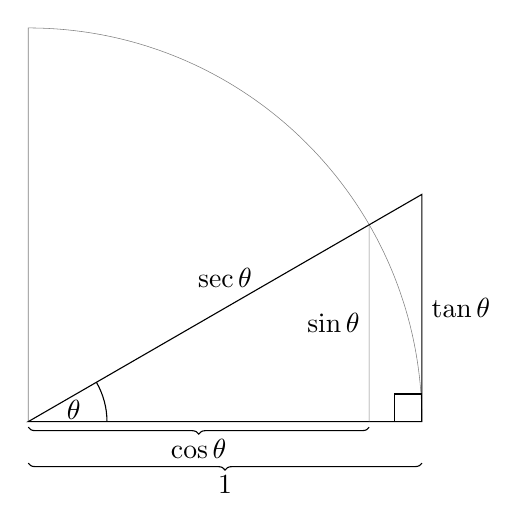
\begin{tikzpicture}[scale=5]
  \coordinate (A) at (0, 0);
  \coordinate (B) at (30:1);
  \coordinate (C) at (B |- {(1, 0)});
  \coordinate (Bsec) at (30:{sec(30)});
  \coordinate (Csec) at (1, 0);

  \draw[help lines] (0, 1) -- (0, 0) --
    (1, 0) arc [start angle=0, end angle=90, radius=1] -- cycle;

  \draw (A) -- node[above, yshift=4pt] {$\sec\theta$}
    (Bsec) -- node[right] {$\tan\theta$}
    (Csec) -- cycle;

  \draw[help lines] (B) -- node[left, text=black] {$\sin\theta$} (C);
  \draw[decorate, decoration={brace, raise=2pt}] (C) -- (A)
    node[midway, below=3pt] {$\cos\theta$};
  \draw[decorate, decoration={brace, raise=15pt}] (Csec) -- (A)
    node[midway, below=16pt] {$1$};

  \draw pic[angle radius=10mm, draw=black, "$\theta$"] {angle=C--A--B};
  \draw (Csec) rectangle +(-2pt, 2pt);
\end{tikzpicture}
\end{document}

%%% Local Variables:
%%% mode: latex
%%% TeX-master: t
%%% End:
